
%%%%%%%%%%%%%%%%%%%%%%% file typeinst.tex %%%%%%%%%%%%%%%%%%%%%%%%%
%
% This is the LaTeX source for the instructions to authors using
% the LaTeX document class 'llncs.cls' for contributions to
% the Lecture Notes in Computer Sciences series.
% http://www.springer.com/lncs       Springer Heidelberg 2006/05/04
%
% It may be used as a template for your own input - copy it
% to a new file with a new name and use it as the basis
% for your article.
%
% NB: the document class 'llncs' has its own and detailed documentation, see
% ftp://ftp.springer.de/data/pubftp/pub/tex/latex/llncs/latex2e/llncsdoc.pdf
%
%%%%%%%%%%%%%%%%%%%%%%%%%%%%%%%%%%%%%%%%%%%%%%%%%%%%%%%%%%%%%%%%%%%


\documentclass[runningheads,a4paper]{llncs}

\usepackage{amssymb}
\setcounter{tocdepth}{3}
\usepackage{graphicx}

\usepackage{url}
\urldef{\mailsa}\path|{alfred.hofmann, ursula.barth, ingrid.haas, frank.holzwarth,|
\urldef{\mailsb}\path|anna.kramer, leonie.kunz, christine.reiss, nicole.sator,|
\urldef{\mailsc}\path|erika.siebert-cole, peter.strasser, lncs}@springer.com|    
\newcommand{\keywords}[1]{\par\addvspace\baselineskip
\noindent\keywordname\enspace\ignorespaces#1}

\begin{document}

\mainmatter  % start of an individual contribution

% first the title is needed
\title{Automated Election Auditing of DRE Audit Logs}

% a short form should be given in case it is too long for the running head
\titlerunning{Automated Analysis of Election Audit Logs}

% the name(s) of the author(s) follow(s) next
%
% NB: Chinese authors should write their first names(s) in front of
% their surnames. This ensures that the names appear correctly in
% the running heads and the author index.
%
\author{Patrick Baxter
\and Anne Edmundson\and Keishla Ortiz\and Ana Maria Quevedo\and\\
Samuel Rodr\'{i}guez\and Cynthia Sturton\and David Wagner}
%
\authorrunning{Automated Analysis of Election Audit Logs}
% (feature abused for this document to repeat the title also on left hand pages)

% the affiliations are given next; don't give your e-mail address
% unless you accept that it will be published
\institute{Springer-Verlag, Computer Science Editorial,\\
Tiergartenstr. 17, 69121 Heidelberg, Germany\\
\mailsa\\
\mailsb\\
\mailsc\\
\url{http://www.springer.com/lncs}}

%
% NB: a more complex sample for affiliations and the mapping to the
% corresponding authors can be found in the file "llncs.dem"
% (search for the string "\mainmatter" where a contribution starts).
% "llncs.dem" accompanies the document class "llncs.cls".
%

\toctitle{Lecture Notes in Computer Science}
\tocauthor{Authors' Instructions}
\maketitle


%Changes here (in the main paper I'll just invoke this file)
\subsection*{Abstract}
Voting audit logs, produced by electronic voting systems, contain information that is useful for uncovering procedural errors and election anomalies, but are currently unwieldy and hard for election officials to use in post-election audits.  We have devised a way to make the auditing process quick and efficient for election officials.  In order to audit elections, we develop new techniques for detecting equipment problems and procedural mistakes made by election workers; we have automated these analyses for a user-friendly process.  We implemented our methods and built a website for this tool that has the capability of analyzing electronic voting machine log files.  We intend for this work to assist those working with election auditing to quickly identify voting equipment or procedural issues and correct them before election results are certified.  Such issues include locating voting machines or media containing vote data that have not been included in the aggregated count, and voting equipment that needs maintenance before the next election.

\bigvertspace
\section{Introduction}
\smvertspace
A DRE is a type of electronic voting machine in which the
voter interacts directly with the machine, typically through a touch
screen. DREs provide a friendly interface to assist the voter with the
ballot marking process. Similar to the commonly used optical scan
systems, DRE units can reduce overvoting and undervoting. Uniquely,
DRE machines can issue electronic ballots on demand; running out of
paper ballots is no longer an issue. Additionally, audio DREs can
assist visually impaired voters.
 
Federal standards require that electronic voting machines generate
detailed audit logs, which can be used during post-election
audits. These logs record events as they occur on the voting machine 
such as opening the machine for voting, casting a vote or closing the
machine at the end of election day. The log data may also include a
record of every ballot cast in the voting machine.  Previous work has
shown how these logs can be analyzed to uncover procedural errors and
anomalies that occur during the election\cite{Buell2011}.
Unfortunately, manual analysis of raw log data is usually cumbersome
and time consuming, making county-wide post-election analysis
impractical and prone to human error. Therefore, at the present time,
election officials do not regularly perform these types of analyses. 

We aim to make DRE audit log analysis more useful and accessible to
both election officials and other interested parties. In this work, we
develop new methods to analyze these audit logs for the detection of
both procedural errors and system deficiencies. We created a public
web application that applies our methods to detect procedural errors
and system deficiencies.  Election officials can use our tool to
identify memory cartridges containing precinct totals that were not
uploaded on election night, machines that may have experienced
hardware problems during the election, and polling locations that
closed late or had voters waiting in line for extended periods.
 
Our research builds on a similar study that was conducted with DRE audit data collected by fourteen South Carolina counties during the 2010 primary and general elections.  The authors of that study were able to determine, solely by analyzing the audit logs, that 1127 votes did not get included in the official certified tally in Richland County, South Carolina~\cite{Buell2011}. These findings were possible because DRE systems used in South Carolina produce three different types of audit logs, each capturing slightly different information. By cross checking the logs against each other, the authors found inconsistencies that enabled them to uncover the missing votes. In our research we used the same data set as a basis for development of our software. First, we replicated the detection of votes not uploaded. We took this matter further and found fifteen memory devices containing votes that were not uploaded to the tabulation systems from seven counties during the 2010 General election. These memory devices tallied 2082 total votes. Without additional information we could not verify if alternate procedures were used to add these missing votes to the aggregated totals. 

We implement these methods for the ES\&S iVotronic DRE as the 2010 South
Carolina data was already publically available through a previous
Freedom of Information Act request and the iVotronic was used in that election. \cks{Is this true? I changed the wording, but I'm not actually sure
  how the data was made available.} The iVotronic system is a
standalone, portable, touchscreen system that records vote totals,
ballot images and an event log on internal flash 
memory. The event log records, in chronological order, the system
events including unit configuration, polls opened, votes cast, polls
closed, calibration or battery issues, and system errors or warnings. 
iVotronic voting machines represent one of the most widely deployed
DREs in the U.S. In 2010, 422 jurisdictions tallying more than 22
million registered voters used this system~\cite{VerVot2010}. However, our methods for analysis of audit logs
are applicable to all DRE voting systems  that produce the necessary
audit logs.  

A brief description of several problems we detect follows.

\textbf{Votes not uploaded.} We detect  memory cartridges used to close voting machines that have not had their vote data uploaded to the tabulation system. This situation, if not corrected, can result in votes left out of the official results.

\textbf{Machines not closed.} We detect voting machines that were not
closed for voting at the polling location. Failure to close a machine
on election night may result in its votes being left out of the
certified count.

\textbf{Missing terminals from the audit database.} This analysis
identifies voting machines used during the election whose event log or
ballot images have not been uploaded to the election reporting
software. Complete DRE ballot images and event logs will allow for
more accurate post-election audits. 

\textbf{Polling location related analyses.} Our tool provides a series of analyses related to polling location activity. We identify locations that stayed open late as well as locations that may have experienced long lines during the day. This information can help county officials to identify locations that may need additional resources in the future. 

\textbf{DRE voting machine configuration and hardware problems.} Our tool performs several analyses that can identify  voting machines that may need testing, repair or reconfiguration. These analyses include identifying possible calibration issues, machines with potential power supply issues, machines that were forced to close early, and machines with incorrect date and time settings.

\textbf{Poll worker training related issues.} We also identify incorrect procedures at the precincts such as using the wrong cartridge to close the voting machines in a precinct, forgetting to print the precinct's zero tape or activating ballots with the incorrect cartridge. Election officials may be able to use this information to improve poll worker training and minimize recurrences in the future.

In this work we assume that DRE audit logs are complete, accurate,  trustworthy, and free of accidental or malicious tampering. Detecting and preventing audit log tampering is outside of the scope of this work.

In summary, this paper develops and implements new ways that audit log data can be used meaningfully and in an automated fashion to enhance the accuracy and efficiency of elections. We believe our tool will provide useful feedback to election administrators during the canvassing process. We hope that this study illustrates the potential value of voting systems' audit logs and motivates future election technologies to provide enhanced support for these purposes.




\section{Introduction}

You are strongly encouraged to use \LaTeXe{} for the
preparation of your camera-ready manuscript together with the
corresponding Springer class file \verb+llncs.cls+. Only if you use
\LaTeXe{} can hyperlinks be generated in the online version
of your manuscript.

The \LaTeX{} source of this instruction file for \LaTeX{} users may be
used as a template. This is
located in the ``authors'' subdirectory in
\url{ftp://ftp.springer.de/pub/tex/latex/llncs/latex2e/instruct/} and
entitled \texttt{typeinst.tex}. There is a separate package for Word 
users. Kindly send the final and checked source
and PDF files of your paper to the Contact Volume Editor. This is
usually one of the organizers of the conference. You should make sure
that the \LaTeX{} and the PDF files are identical and correct and that
only one version of your paper is sent. It is not possible to update
files at a later stage. Please note that we do not need the printed
paper.

We would like to draw your attention to the fact that it is not possible
to modify a paper in any way, once it has been published. This applies
to both the printed book and the online version of the publication.
Every detail, including the order of the names of the authors, should
be checked before the paper is sent to the Volume Editors.

\subsection{Checking the PDF File}

Kindly assure that the Contact Volume Editor is given the name and email
address of the contact author for your paper. The Contact Volume Editor
uses these details to compile a list for our production department at
SPS in India. Once the files have been worked upon, SPS sends a copy of
the final pdf of each paper to its contact author. The contact author is
asked to check through the final pdf to make sure that no errors have
crept in during the transfer or preparation of the files. This should
not be seen as an opportunity to update or copyedit the papers, which is
not possible due to time constraints. Only errors introduced during the
preparation of the files will be corrected.

This round of checking takes place about two weeks after the files have
been sent to the Editorial by the Contact Volume Editor, i.e., roughly
seven weeks before the start of the conference for conference
proceedings, or seven weeks before the volume leaves the printer's, for
post-proceedings. If SPS does not receive a reply from a particular
contact author, within the timeframe given, then it is presumed that the
author has found no errors in the paper. The tight publication schedule
of LNCS does not allow SPS to send reminders or search for alternative
email addresses on the Internet.

In some cases, it is the Contact Volume Editor that checks all the final
pdfs. In such cases, the authors are not involved in the checking phase.

\subsection{Additional Information Required by the Volume Editor}

If you have more than one surname, please make sure that the Volume Editor
knows how you are to be listed in the author index.

\subsection{Copyright Forms}

The copyright form may be downloaded from the ``For Authors"
(Information for LNCS Authors) section of the LNCS Website:
\texttt{www.springer.com/lncs}. Please send your signed copyright form
to the Contact Volume Editor, either as a scanned pdf or by fax or by
courier. One author may sign on behalf of all of the other authors of a
particular paper. Digital signatures are acceptable.

\section{Paper Preparation}

Springer provides you with a complete integrated \LaTeX{} document class
(\texttt{llncs.cls}) for multi-author books such as those in the LNCS
series. Papers not complying with the LNCS style will be reformatted.
This can lead to an increase in the overall number of pages. We would
therefore urge you not to squash your paper.

Please always cancel any superfluous definitions that are
not actually used in your text. If you do not, these may conflict with
the definitions of the macro package, causing changes in the structure
of the text and leading to numerous mistakes in the proofs.

If you wonder what \LaTeX{} is and where it can be obtained, see the
``\textit{LaTeX project site}'' (\url{http://www.latex-project.org})
and especially the webpage ``\textit{How to get it}''
(\url{http://www.latex-project.org/ftp.html}) respectively.

When you use \LaTeX\ together with our document class file,
\texttt{llncs.cls},
your text is typeset automatically in Computer Modern Roman (CM) fonts.
Please do
\emph{not} change the preset fonts. If you have to use fonts other
than the preset fonts, kindly submit these with your files.

Please use the commands \verb+\label+ and \verb+\ref+ for
cross-references and the commands \verb+\bibitem+ and \verb+\cite+ for
references to the bibliography, to enable us to create hyperlinks at
these places.

For preparing your figures electronically and integrating them into
your source file we recommend using the standard \LaTeX{} \verb+graphics+ or
\verb+graphicx+ package. These provide the \verb+\includegraphics+ command.
In general, please refrain from using the \verb+\special+ command.

Remember to submit any further style files and
fonts you have used together with your source files.

\subsubsection{Headings.}

Headings should be capitalized
(i.e., nouns, verbs, and all other words
except articles, prepositions, and conjunctions should be set with an
initial capital) and should,
with the exception of the title, be aligned to the left.
Words joined by a hyphen are subject to a special rule. If the first
word can stand alone, the second word should be capitalized.

Here are some examples of headings: ``Criteria to Disprove
Context-Freeness of Collage Language", ``On Correcting the Intrusion of
Tracing Non-deterministic Programs by Software", ``A User-Friendly and
Extendable Data Distribution System", ``Multi-flip Networks:
Parallelizing GenSAT", ``Self-determinations of Man".

\subsubsection{Lemmas, Propositions, and Theorems.}

The numbers accorded to lemmas, propositions, and theorems, etc. should
appear in consecutive order, starting with Lemma 1, and not, for
example, with Lemma 11.

\subsection{Figures}

For \LaTeX\ users, we recommend using the \emph{graphics} or \emph{graphicx}
package and the \verb+\includegraphics+ command.

Please check that the lines in line drawings are not
interrupted and are of a constant width. Grids and details within the
figures must be clearly legible and may not be written one on top of
the other. Line drawings should have a resolution of at least 800 dpi
(preferably 1200 dpi). The lettering in figures should have a height of
2~mm (10-point type). Figures should be numbered and should have a
caption which should always be positioned \emph{under} the figures, in
contrast to the caption belonging to a table, which should always appear
\emph{above} the table; this is simply achieved as matter of sequence in
your source.

Please center the figures or your tabular material by using the \verb+\centering+
declaration. Short captions are centered by default between the margins
and typeset in 9-point type (Fig.~\ref{fig:example} shows an example).
The distance between text and figure is preset to be about 8~mm, the
distance between figure and caption about 6~mm.

To ensure that the reproduction of your illustrations is of a reasonable
quality, we advise against the use of shading. The contrast should be as
pronounced as possible.

If screenshots are necessary, please make sure that you are happy with
the print quality before you send the files.
%\begin{figure}
%\centering
%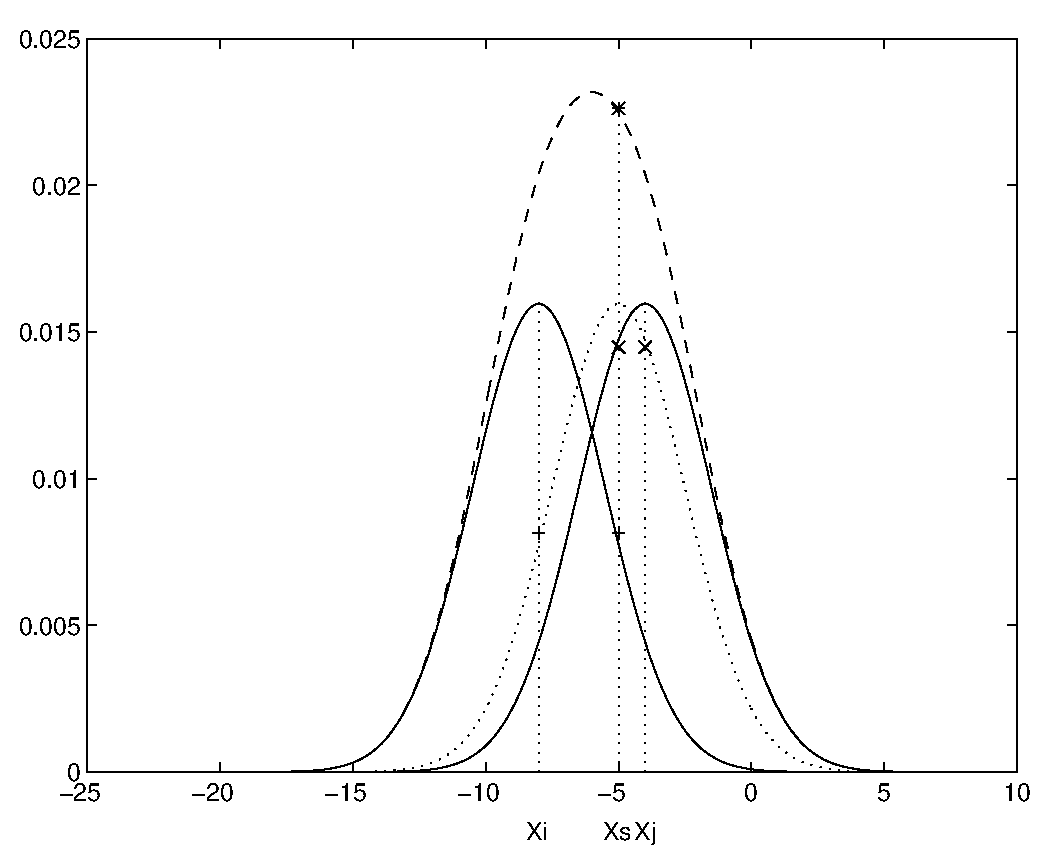
\includegraphics[height=6.2cm]{eijkel2.eps}
%\caption{One kernel at $x_s$ (\emph{dotted kernel}) or two kernels at
%$x_i$ and $x_j$ (\textit{left and right}) lead to the same summed estimate
%at $x_s$. This shows a figure consisting of different types of
%lines. Elements of the figure described in the caption should be set in
%italics, in parentheses, as shown in this sample caption.}
%\label{fig:example}
%\end{figure}

Please define figures (and tables) as floating objects. Please avoid
using optional location parameters like ``\verb+[h]+" for ``here".

\paragraph{Remark 1.}

In the printed volumes, illustrations are generally black and white
(halftones), and only in exceptional cases, and if the author is
prepared to cover the extra cost for color reproduction, are colored
pictures accepted. Colored pictures are welcome in the electronic
version free of charge. If you send colored figures that are to be
printed in black and white, please make sure that they really are
legible in black and white. Some colors as well as the contrast of
converted colors show up very poorly when printed in black and white.

\subsection{Formulas}

Displayed equations or formulas are centered and set on a separate
line (with an extra line or halfline space above and below). Displayed
expressions should be numbered for reference. The numbers should be
consecutive within each section or within the contribution,
with numbers enclosed in parentheses and set on the right margin --
which is the default if you use the \emph{equation} environment, e.g.,
\begin{equation}
  \psi (u) = \int_{o}^{T} \left[\frac{1}{2}
  \left(\Lambda_{o}^{-1} u,u\right) + N^{\ast} (-u)\right] dt \;  .
\end{equation}

Equations should be punctuated in the same way as ordinary
text but with a small space before the end punctuation mark.

\subsection{Footnotes}

The superscript numeral used to refer to a footnote appears in the text
either directly after the word to be discussed or -- in relation to a
phrase or a sentence -- following the punctuation sign (comma,
semicolon, or period). Footnotes should appear at the bottom of
the
normal text area, with a line of about 2~cm set
immediately above them.\footnote{The footnote numeral is set flush left
and the text follows with the usual word spacing.}

\subsection{Program Code}

Program listings or program commands in the text are normally set in
typewriter font, e.g., CMTT10 or Courier.

\medskip

\noindent
{\it Example of a Computer Program}
\begin{verbatim}
program Inflation (Output)
  {Assuming annual inflation rates of 7%, 8%, and 10%,...
   years};
   const
     MaxYears = 10;
   var
     Year: 0..MaxYears;
     Factor1, Factor2, Factor3: Real;
   begin
     Year := 0;
     Factor1 := 1.0; Factor2 := 1.0; Factor3 := 1.0;
     WriteLn('Year  7% 8% 10%'); WriteLn;
     repeat
       Year := Year + 1;
       Factor1 := Factor1 * 1.07;
       Factor2 := Factor2 * 1.08;
       Factor3 := Factor3 * 1.10;
       WriteLn(Year:5,Factor1:7:3,Factor2:7:3,Factor3:7:3)
     until Year = MaxYears
end.
\end{verbatim}
%
\noindent
{\small (Example from Jensen K., Wirth N. (1991) Pascal user manual and
report. Springer, New York)}

\subsection{Citations}

For citations in the text please use
square brackets and consecutive numbers: \cite{jour}, \cite{lncschap},
\cite{proceeding1} -- provided automatically
by \LaTeX 's \verb|\cite| \dots\verb|\bibitem| mechanism.

\subsection{Page Numbering and Running Heads}

There is no need to include page numbers. If your paper title is too
long to serve as a running head, it will be shortened. Your suggestion
as to how to shorten it would be most welcome.

\section{LNCS Online}

The online version of the volume will be available in LNCS Online.
Members of institutes subscribing to the Lecture Notes in Computer
Science series have access to all the pdfs of all the online
publications. Non-subscribers can only read as far as the abstracts. If
they try to go beyond this point, they are automatically asked, whether
they would like to order the pdf, and are given instructions as to how
to do so.

Please note that, if your email address is given in your paper,
it will also be included in the meta data of the online version.

\section{BibTeX Entries}

The correct BibTeX entries for the Lecture Notes in Computer Science
volumes can be found at the following Website shortly after the
publication of the book:
\url{http://www.informatik.uni-trier.de/~ley/db/journals/lncs.html}

\subsubsection*{Acknowledgments.} The heading should be treated as a
subsubsection heading and should not be assigned a number.

\bibliographystyle{plain}
\bibliography{paper2}


\section*{Appendix: Springer-Author Discount}
LNCS authors are entitled to a 33.3\% discount off all Springer
publications. Before placing an order, the author should send an email, 
giving full details of his or her Springer publication,
to \url{orders-HD-individuals@springer.com} to obtain a so-called token. This token is a
number, which must be entered when placing an order via the Internet, in
order to obtain the discount.

\end{document}
